\documentclass{article}

\usepackage[shellescape]{gmp}
\usepackage[utf8]{inputenc}
\usepackage{german}

\usepackage{geometry}
\geometry{margin=2cm,tmargin=2.5cm,bmargin=2cm}

\usepackage{graphicx}
\DeclareGraphicsRule{*}{mps}{*}{}

\usepackage{pdflscape}

\usepackage{titling}
\setlength{\droptitle}{80px}

\usepackage{xcolor}
\definecolor{light-gray}{gray}{0.95}
\definecolor{gold}{HTML}{FFD700}
\definecolor{vared}{HTML}{BF0020}
\usepackage{nicefrac}

\usepackage[nopostdot]{glossaries}
\makeglossaries
\loadglsentries{glossary}

\usepackage{soul}

\usepackage[colorlinks=true,urlcolor=blue]{hyperref}

\renewcommand{\figurename}{Abbildung}

\begin{document}
\title{\Large Einsendeaufgabe \\ Analyse}
\author{\normalsize Stefan Berger}
\date{}
\maketitle

\vspace{160px}

\pagebreak

\section{Unternehmensziele}
\paragraph{}
Zur Mehrung des Gewinns soll der Bekanntheitsgrad bei Onlineshops, \gls{portal}en und Käufern gesteigert werden. Bis einen Monat nach Abschluss dieses Projekts sollen 350 neue Partner hinzukommen.
\paragraph{}
Je nach Intensität der Nutzung der \gls{sw} sollen Partner eine Nutzungsgebühr in Höhe von 30 bis 150 Euro monatlich zahlen. Die geschätzten Projektkosten von 45 000 Euro sollen sich nach 9 bis 10 Jahren amortisiert haben. Das übrige Budget von 1 550 000 Euro ist für die Gehaltskosten des Vertriebspersonals und für das Marketing vorgesehen.

\section{Vision und Systemidee}
{
  \centering
  \noindent\fcolorbox{gray}{light-gray}{%
          \textit{Die \gls{sw} soll den Kunden von Onlineshops einen differenzierten Eindruck der Produkte vermitteln.}
  }

}

\paragraph{}
Ziel des Projektes ist es, Onlinehändler durch eine webbasierte \gls{sw} zu verbinden, mit der Produktreviews mit Punktwertung (1-5 Sterne), Beschreibungen und Übersetzungen der Beschreibungen erstellt und geteilt werden können.

\begin{figure}[h]
  \centering
  
\includegraphics[scale=0.5]{logo.png}
  \caption{Vorschlag für ein Logo}
  \label{logo}
\end{figure}

\paragraph{}
Vorschlag für einen Slogan: \textit{Buy aware!}

\section{Fachwissen}
\paragraph{}
Onlineshops und \gls{portal}e betreiben immer eine oder mehrere Webseiten, die auf HTTP und HTML basieren. Die Webauftritte können durch native Mobile-Apps ergänzt werden. Die \gls{sw} soll möglichst direkt mit allen Webseiten und -anwendungen der Händler und Portale genutzt werden können.

\paragraph{}
Die zu bewertenden Verkaufsartikel können durch \gls{feed}s aus den Produktdatenbanken der Onlineshops exportiert und in den Datenbestand der \gls{portal}e importiert werden. Die Feeds beinhalten pro Artikel einen Stock-Keeping-Unit-Code (\gls{sku}), durch den das Produkt eines Shops plattformübergreifend eindeutig identifiziert werden kann. Die Identifikation eines Artikels in \gls{feed}s von verschiedenen Onlineshops ist nur in wenigen Produktkategorien möglich, etwa mittels ISBN bei Büchern oder Herstellernamen und Modellnummer bei Elektrogeräten.

\paragraph{}
Die \gls{sw} benötigt einen eigenen Produktdatenbestand, um den Produkten die jeweiligen \gls{review}s zuzuordnen. Hierfür muss ein flexibler Datenimport implementiert werden, da die \gls{feed}s der Onlineshops in verschiedensten Formaten (CSV mit unterschiedlichen Trennzeichen, XML mit unterschiedlichen Strukturen usw.) vorliegen.

\section{Marktanalyse}
Alle \gls{portal}e besitzen ein Bewertungssystem für Produkte. Die Systeme von amazon.de und trustedshops.de sind am ausgereiftesten. Bei Amazon können Kunden befragt werden, die ein Produkt bereits früher gekauft haben. Amazon und Trusted Shops nutzen die Kenntnis über den tatsächlichen Kauf eines Produkts, um die Echtheit einer Bewertung zu verifizieren. Da die Portale normalerweise schon über \gls{review}systeme verfügen, ist die Konkurrenz erheblich.

\paragraph{}
Von 10 stichprobenartig ausgewählten Onlineshops besaß mytoys.de als einziger ein eigenes System für Produktbewertungen. Es heißt \glqq KombiShopping\grqq, besitzt noch deutlich mehr Funktionalität und wird außerdem noch in drei anderen Onlineshops desselben Unternehmens genutzt.

\paragraph{}
Die Zielgruppe der \gls{sw} sind hauptsächlich \gls{portal}e. Es gibt eine große Auswahl \gls{portal}e in verschiedenen Branchen, wie etwa Telefon/Internet, Versicherungen, Elektronikprodukte und andere. Zusätzlich gibt es branchenübergreifende \gls{portal}e, wie amazon.de, billiger.de usw.

\section{Stakeholder}
Die \gls{sw} soll von Internetunternehmern auf deren Webseiten nutzbar sein. Die Webseiten aggregieren Angebote von Onlineshops oder anderen kommerziellen Anbietern, die online genutzt werden (E-Commerce).

\section{Interessen der Stakeholder} Der Nutzen für die Stakeholder ergibt sich aus der gesteigerten Bekanntheit der Produkte, den gesteigerten Konvertierungen z.B. bei Webseitenbesuchern von bezahlten Werbelinks, und aus selteneren Rücksendungen wegen Nichtgefallen.

\section{Geschäftsklassen}
\paragraph{}
Die wichtigsten Geschäftsklassen sind \\

\begin{tabular}{|l|l|}
  \hline
  \gls{review} & Beschreibung, Produktbewertung, Verfasser und Alter des \gls{review}s \\
  \hline
  Product & Produktname und Liste mit \gls{review}s \\
  \hline
  Merchant & Verkäufer eines Produkts bzw. zahlender Nutzer der \gls{sw} \\
  \hline
  Customer & Käufer der Produkte und Verfasser der \gls{review}s \\
  \hline
\end{tabular}

\paragraph{}
Die Geschäftsklassen sind auch im UML-Klassendiagramm beschrieben.

\section{Anwendungsfälle und Abläufe}
\paragraph{}
Die Anwendungsfälle und Abläufe sind als Abnahmekriterien auf Karten notiert. Im Einzelnen sind das
\begin{itemize}
  \item Objekte von Geschäftsklassen in Datenbanken speichern
  \item Benutzern der \gls{sw} können die Rechte \glqq \gls{review} schreiben\grqq, \glqq \gls{review} duplizieren\grqq\ und \glqq Rechte vergeben\grqq\ erteilt werden
  \item Objekte von Geschäftsklassen in Datenbanken speichern
  \item Benutzern der \gls{sw} können die Rechte „\gls{review} lesen“, „\gls{review} schreiben“ und „Rechte vergeben“ erteilt werden
  \item Objekte von Geschäftsklassen via  REST Service abfragen und erstellen (nur authentifizierte Benutzer)
  \item \gls{client} des REST-Services als HTML-Snippet
  \item \gls{client} des REST-Services als Desktop-Anwendung
\end{itemize}

\pagebreak

\section{GUI}
\paragraph{}
Die Benutzeroberfläche für die Anzeige von \gls{review}s soll wie abgebildet aussehen (Entwurf):
\begin{figure}[h]
  \centering
  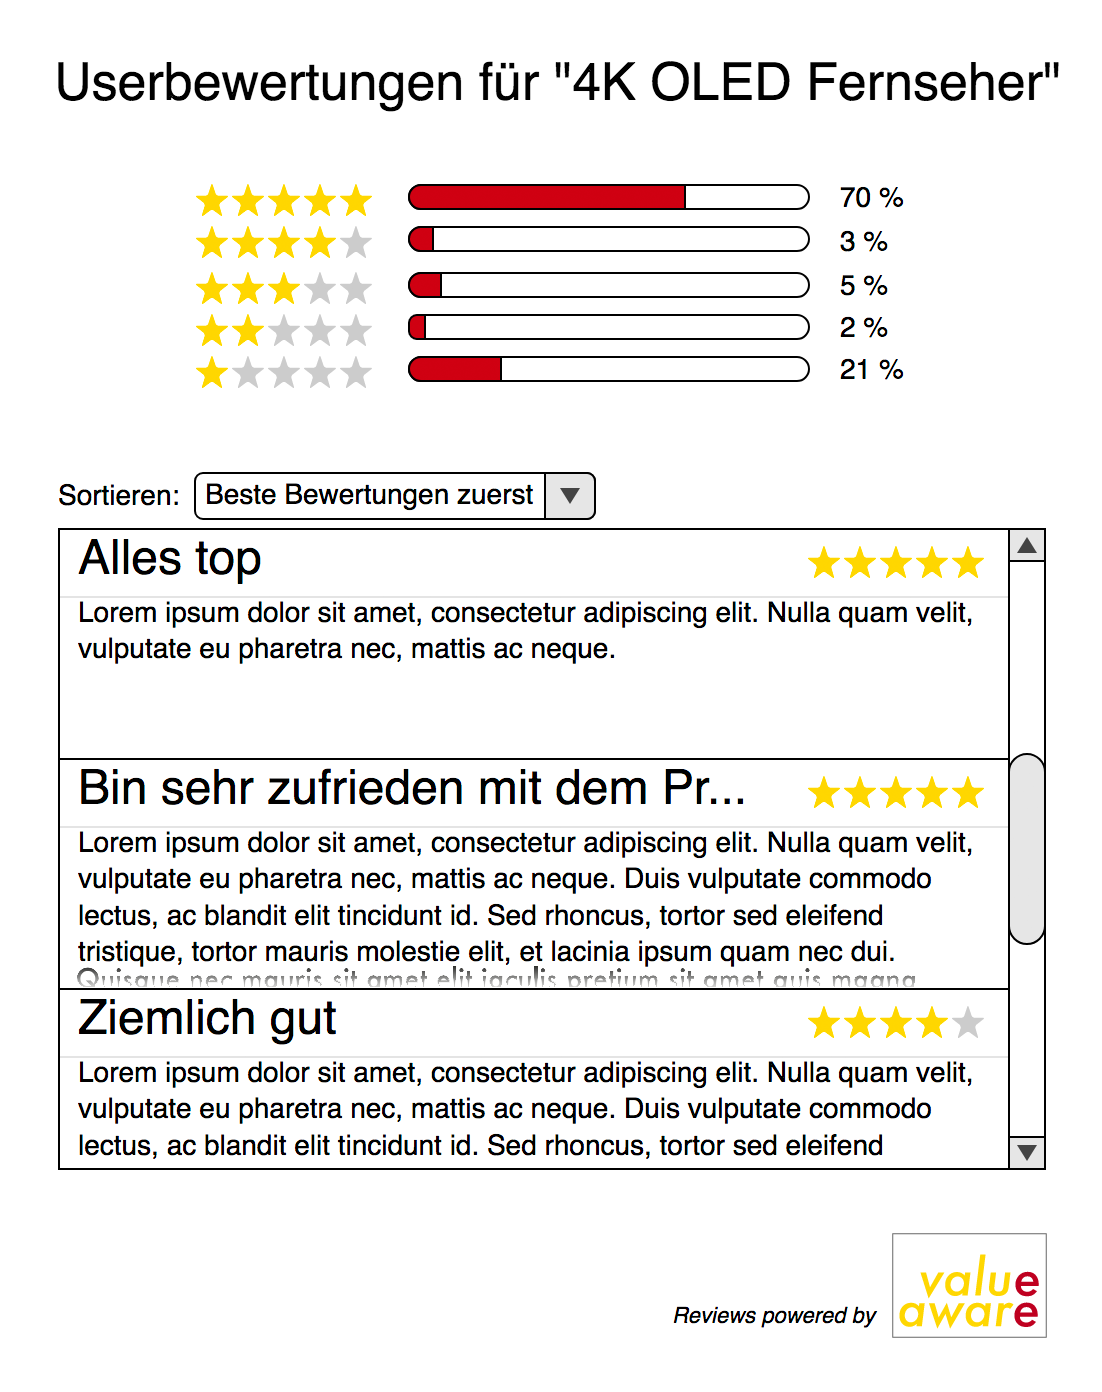
\includegraphics[scale=.35]{review-snippet.png}
  \caption{Designbeispiel für das HTML-Snippet}
  \label{review}
\end{figure}

\pagebreak

\paragraph{}
Die Eingabemaske für Kundenbewertungen sollte etwa so aussehen:

\begin{figure}[h]
  \centering
  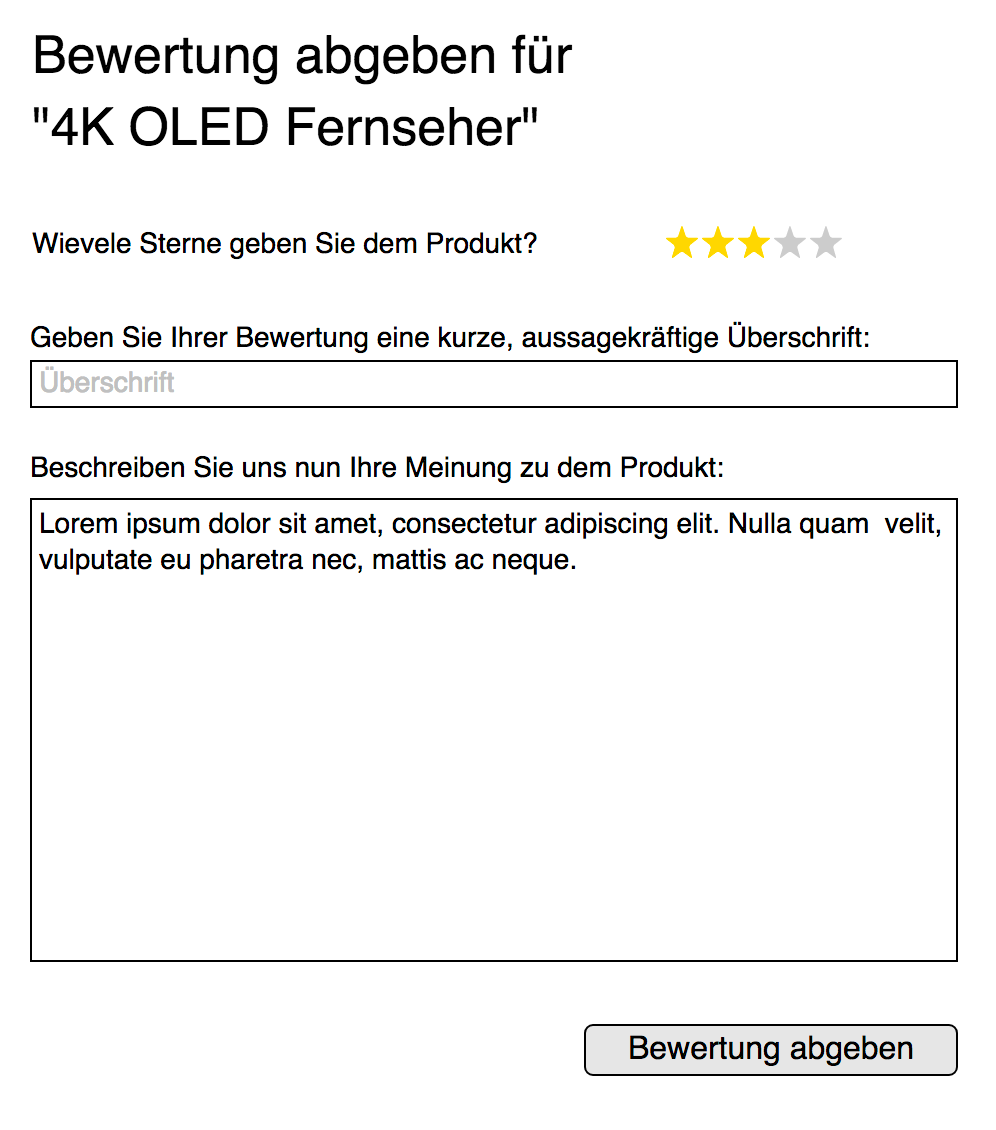
\includegraphics[scale=.3]{review-enter-snippet.png}
  \caption{Designbeispiel für die \gls{review}-Eingabemaske}
  \label{}
\end{figure}

\section{Vorgehensmodel}
\paragraph{}
Die \gls{sw} soll iterativ und in ständiger Zusammenarbeit mit dem Auftraggeber entwickelt werden. Es wird ein Team aus Scrum-Master, Product Owner und 6-8 Entwicklern zusammengestellt. Die Anforderungen werden zusammen mit dem Product Owner als User Stories verfasst und anschließend dem Entwicklerteam vorgestellt. Die Entwickler geben eine erste Schätzung zur Komplexität bzw. Zeitaufwand an. Anschließend können zu große Stories in kleinere aufgeteilt werden.
\paragraph{}
Nach der ersten Iteration (Sprint) soll ein \gls{webservice} \gls{review}s im JSON-Format ausliefern, und eine Webseite diese \gls{review}s anzeigen können. Außerdem soll eine beispielhafte Integration des HTML-Snippets in eine Android- oder iOS-App vorliegen.

\section{Durchführbarkeitsstudie und Risikoanalyse}
\paragraph{}
Das Projekt ist realisierbar. Die Kosten für Hardware und Personal sind vom Budget abgedeckt. Es sollten frühzeitig Führungskräfte (Scrum Master, Product Owner) und Entwickler eingestellt werden. Die zu verwendenden Technologien sind erprobt und unter Entwicklern gut bekannt. Das Projekt kann bereits wenige Monate nach Abschluss der Entwicklung wirtschaftlich erfolgreich sein, sofern ausreichend Kunden akquiriert werden. Es werden ab dem ersten Monat etwa 350 Kunden benötigt, die monatlich 60 Euro für die Nutzung der \gls{sw} zahlen. Das Projekt wird sich dadurch nach etwa 9 Jahren amortisieren. Die Kundenakquise und Kundenbindung sind daher genau zu kontrollieren.

\paragraph{}
Mangelnde Abdeckung der \gls{review}s z.B. pro Produktkategorie könnte einen Negativfaktor der Nachfrage darstellen. Die Abdeckung sollte jeweils mindestens \nicefrac{3}{4} der Anzahl der Produkte in den Kategorien, beziehungsweise durchschnittlich 0,75 \gls{review}s pro Produkt betragen. Dasselbe Mindestverhältnis ist für Übersetzungen anzusetzen.

\paragraph{}
Der Import von \gls{review}s aus anderen Systemen und der die Einbindung der Snippets in die Webseiten und Apps der Kunden könnten eventuell technische Schwierigkeiten hervorbringen. Die Kunden müssen bei diesen Aufgaben gegebenenfalls unterstützt werden.

\section{Qualitätssicherung}
Um die Qualität der Implementierungen sicherzustellen ist  eine Testabdeckung für Unit-Tests von 80\% zu erreichen. Die Benutzeroberflächen, insbesondere das HTML-Snippet, sind in allen wichtigen Browsern zu testen. Hierfür sind End-to-End-Tests vorgesehen. Alle Tests sind zu automatisieren. Die \gls{sw} muss nach jeder Iteration alle Tests erfolgreich durchlaufen.

\section{Systemschnittstelle}
\paragraph{}
Der \gls{webservice} gibt \gls{review}s im JSON-Format aus. Eine Erweiterung um SOAP/XML-Endpoints ist zurzeit nicht geplant. Der \gls{webservice} soll dem Level 3 des Richardson Maturity Models (Hypermedia) entsprechen. Die Schnittstelle ist so zu dokumentieren, dass Kunden sie ohne Unterstützung des Projektteams nutzen können.

\paragraph{}
Zusätzlich zur Dokumentation werden zwei \gls{client}s des Services bereitgestellt. Die \gls{client}s sind ebenfalls zu dokumentieren. Je nach Art ist die Integration in andere Systeme (HTML-Snippet) oder die Benutzung der Oberfläche (Translation Desktop App) verständlich zu beschreiben.

\pagebreak

\setuldepth{p}
\section{Spike}
\paragraph{}
Ein Prototyp des \gls{webservice}s ist auf \href{http://s-berger-bmio.bplaced.net/4/SWT/ANA}{\ul{http://s-berger-bmio.bplaced.net/4/SWT/ANA}}  zu finden. Der \gls{webservice} liefert Review-Beispiele im JSON-Format:
\begin{figure}[h]
  \centering
  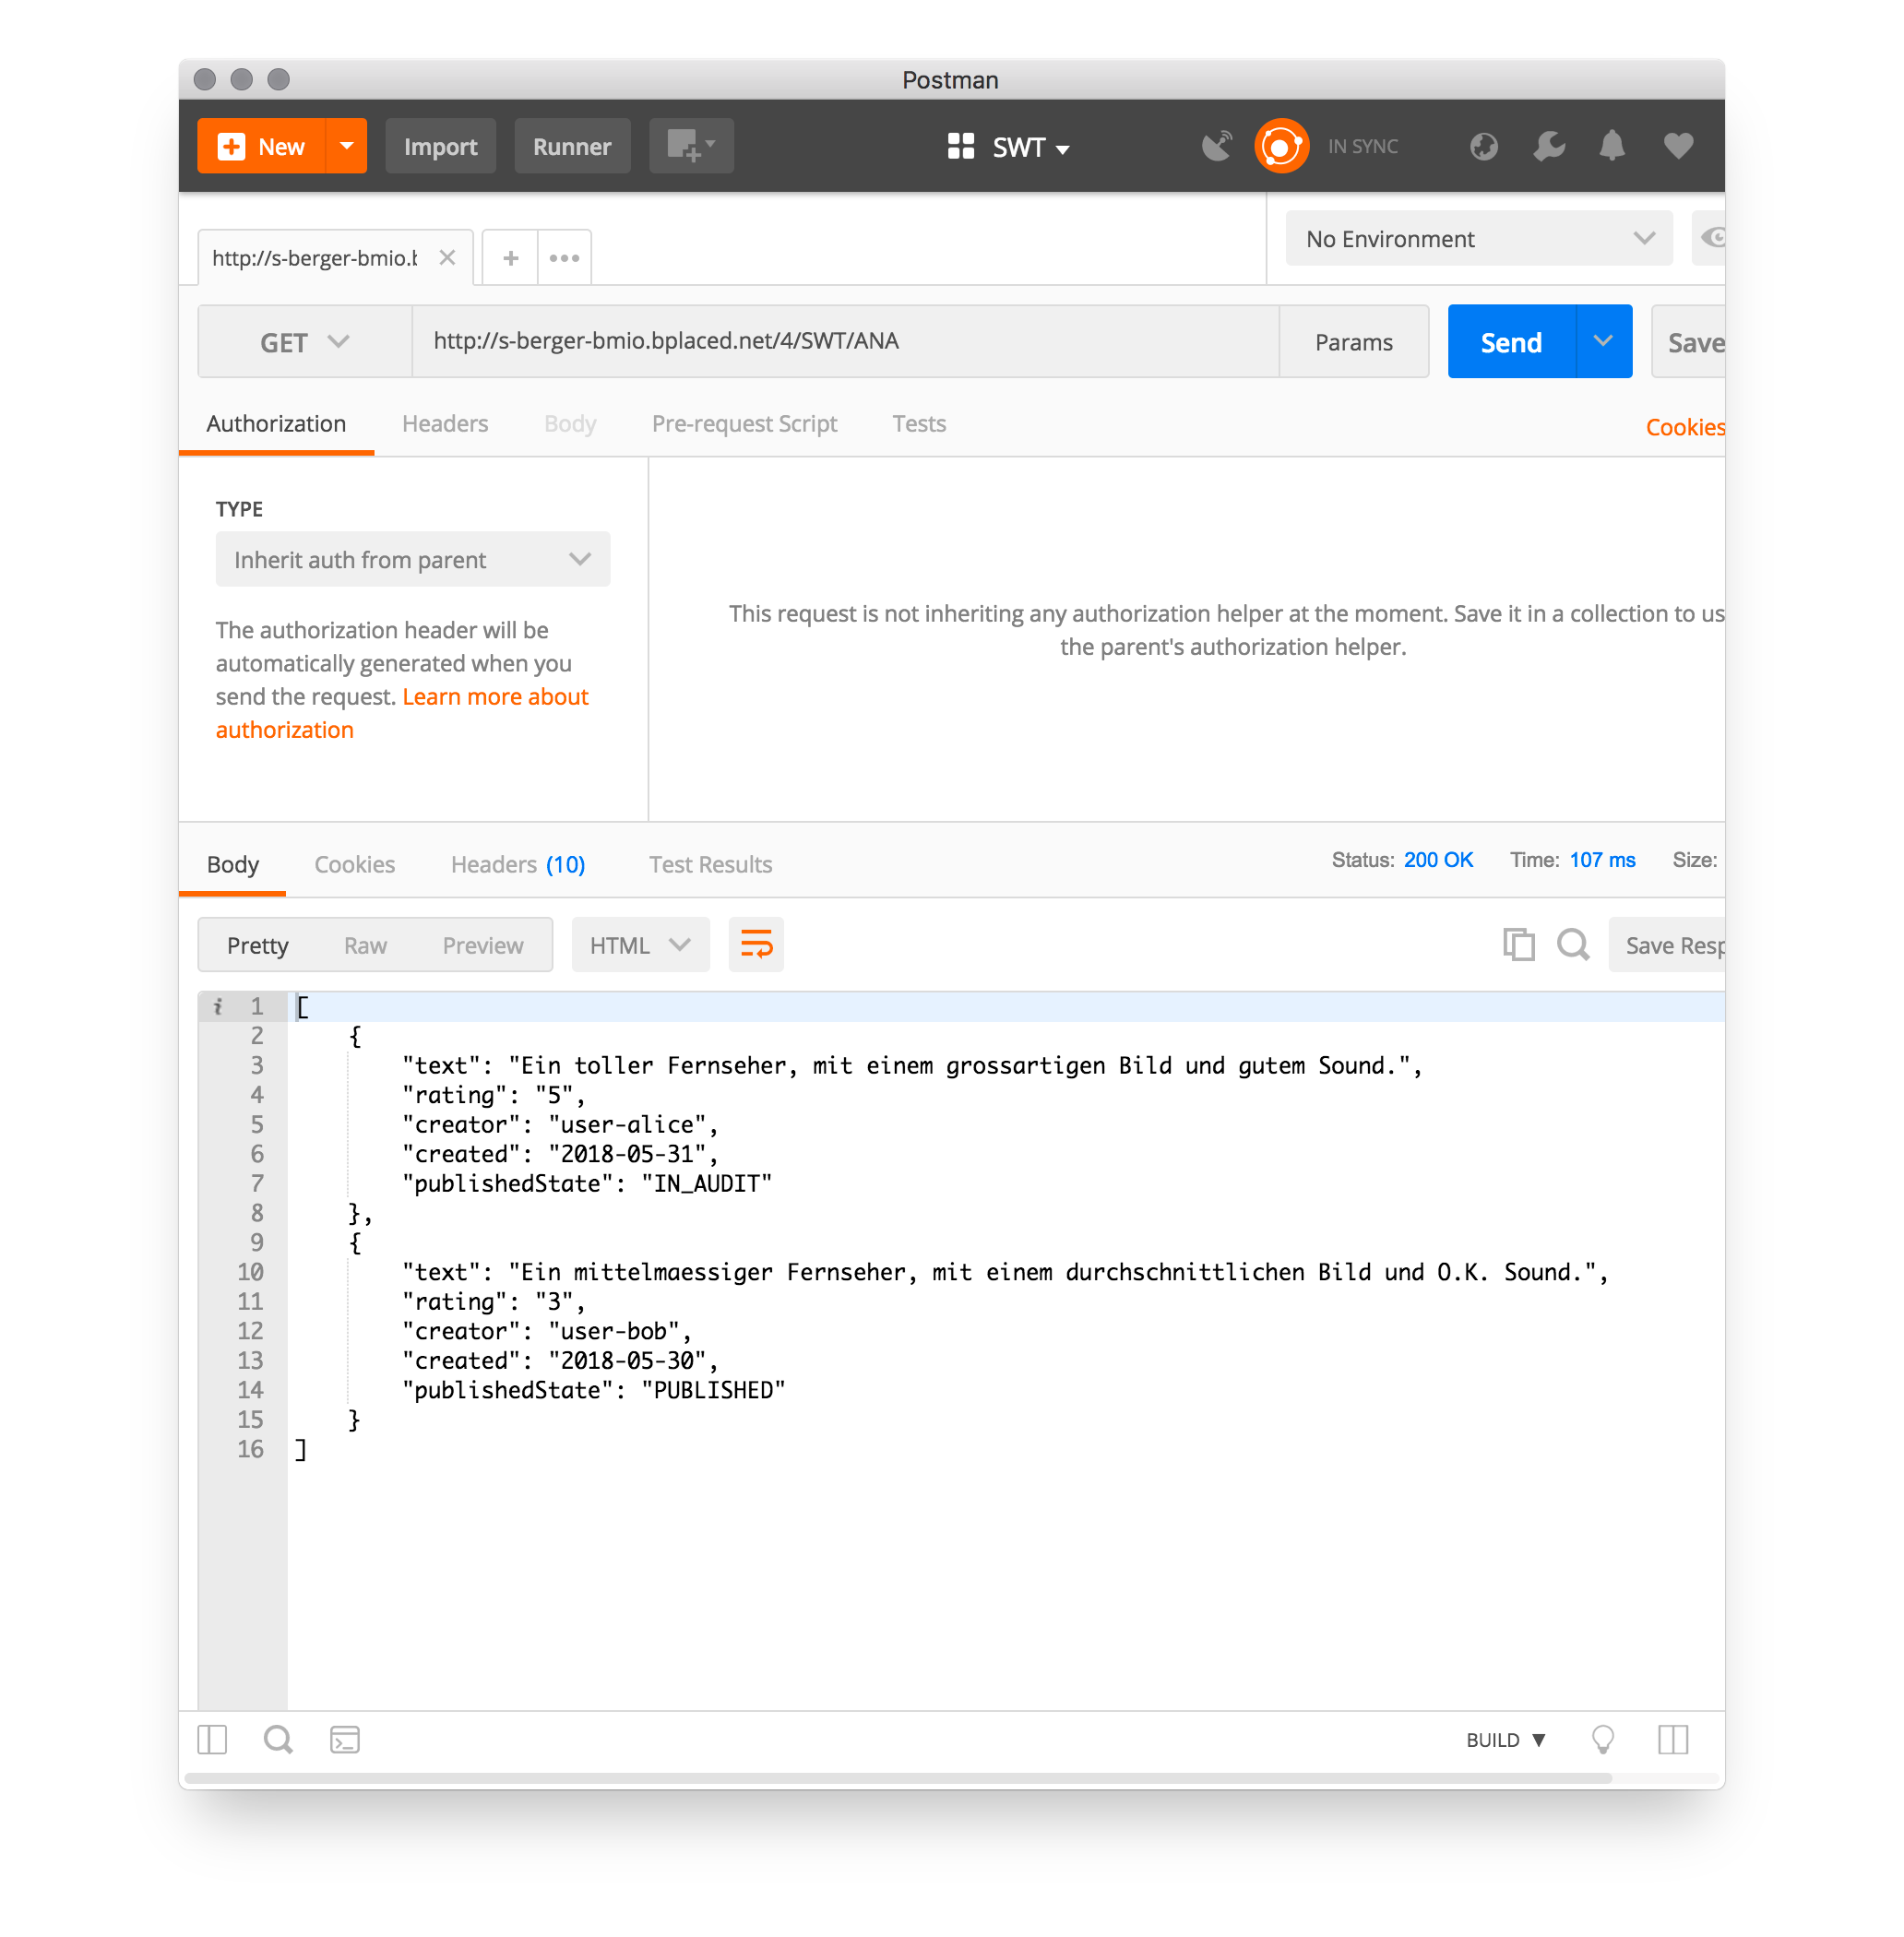
\includegraphics[scale=.2]{spike.png}
  \caption{Screenshot einer Serverantwort des Prototyps}
  \label{spike}
\end{figure}

\pagebreak

\setglossarystyle{altlist}
\printglossary[title=Glossar]

\end{document}
